\documentclass{standalone}
\usepackage{PhysicalChemistryNote}
\begin{document}
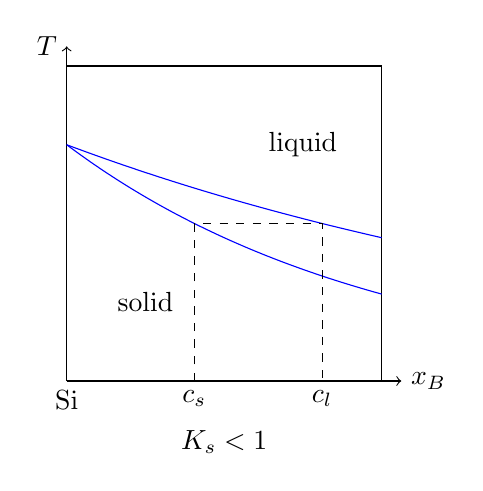
\begin{tikzpicture}
    \draw[->] (0,0) -- (4.25,0) node[right] {$x_B$};
    \draw[->] (0,0) -- (0,4.25) node[left]{$T$};
    \draw[-] (4,0) -- (4,4);
    \draw[-] (0,4) -- (4,4);
    \node[below] at (0,0) {Si};
    \draw[domain=0:4,blue] plot[smooth](\x,{3*e^(-\x/4)});
    \draw[domain=0:4,blue] plot[smooth](\x,{3*e^(-\x/8)});
    \draw[dashed] (1.6218,0)--(1.6218,2)--(3.2437,2)--(3.2437,0);
    \node[below] at (1.6218,0) {$c_{\text s}$};
    \node[below] at (3.2437,0) {$c_{\text l}$};
    \node[below] at (2,-0.5) {$K_s<1$};
    \node at (1,1) {solid};
    \node at (3,3) {liquid};
\end{tikzpicture}
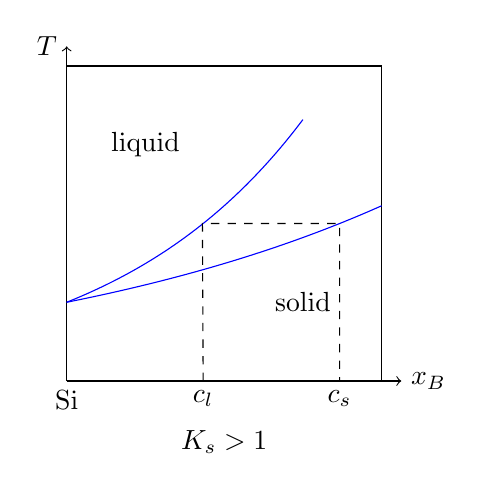
\begin{tikzpicture}
    \draw[->] (0,0) -- (4.25,0) node[right] {$x_B$};
    \draw[->] (0,0) -- (0,4.25) node[left]{$T$};
    \draw[-] (4,0) -- (4,4);
    \draw[-] (0,4) -- (4,4);
    \node[below] at (0,0) {Si};
    \draw[domain=0:3,blue] plot[smooth](\x,{e^(\x/2.5)});
    \draw[domain=0:4,blue] plot[smooth](\x,{e^(\x/5)});
    \draw[dashed] (1.7329,0)--(1.7239,2)--(3.4657,2)--(3.4657,0);
    \node[below] at (1.7329,0) {$c_{\text l}$};
    \node[below] at (3.4657,0) {$c_{\text s}$};
    \node[below] at (2,-0.5) {$K_s>1$};
    \node at (3,1) {solid};
    \node at (1,3) {liquid};
\end{tikzpicture}
\end{document}